
% This file is only the project Overview

\begin{comment}
    ONTENTS OF THE ENTIRE DOCUMENT
    Change History i
    Preface ii
    List of Figures v
    List of Tables vi
    1 Project Overview 1
    2 Project Overview 2
    2.1 Project Description . . . . . . . . . . . . . . . . . . . . . . . . . . . . . . . . . . . . 2
    3 Project Overview 3
    3.1 Project Description . . . . . . . . . . . . . . . . . . . . . . . . . . . . . . . . . . . . 3
    3.1.1 Background . . . . . . . . . . . . . . . . . . . . . . . . . . . . . . . . . . . . 3
    3.1.2 Scope . . . . . . . . . . . . . . . . . . . . . . . . . . . . . . . . . . . . . . . 3
    3.1.3 Purpose . . . . . . . . . . . . . . . . . . . . . . . . . . . . . . . . . . . . . . 3
    3.1.4 Objectives (SMART Goals) . . . . . . . . . . . . . . . . . . . . . . . . . . . 4
    3.2 Stakeholders . . . . . . . . . . . . . . . . . . . . . . . . . . . . . . . . . . . . . . . . 4
    3.2.1 Customer: Axis Communications AB . . . . . . . . . . . . . . . . . . . . . 4
    3.2.2 Development Team: Company 3 . . . . . . . . . . . . . . . . . . . . . . . . 4
    3.2.3 End Users . . . . . . . . . . . . . . . . . . . . . . . . . . . . . . . . . . . . . 5
    3.3 Project Constraints . . . . . . . . . . . . . . . . . . . . . . . . . . . . . . . . . . . . 5
    3.3.1 Personnel . . . . . . . . . . . . . . . . . . . . . . . . . . . . . . . . . . . . . 5
    3.3.2 Timeline . . . . . . . . . . . . . . . . . . . . . . . . . . . . . . . . . . . . . . 5
    3.3.3 Resources . . . . . . . . . . . . . . . . . . . . . . . . . . . . . . . . . . . . . 5
    3.4 Deliverables . . . . . . . . . . . . . . . . . . . . . . . . . . . . . . . . . . . . . . . . 6
    3.4.1 Product Deliverables . . . . . . . . . . . . . . . . . . . . . . . . . . . . . . . 6
    3.4.2 Documentation Deliverables . . . . . . . . . . . . . . . . . . . . . . . . . . . 6
    3.5 Project Schedule . . . . . . . . . . . . . . . . . . . . . . . . . . . . . . . . . . . . . 6
    3.5.1 Iteration Plan . . . . . . . . . . . . . . . . . . . . . . . . . . . . . . . . . . . 6
    3.5.2 Key Milestones . . . . . . . . . . . . . . . . . . . . . . . . . . . . . . . . . . 6
    3.6 Quality Objectives . . . . . . . . . . . . . . . . . . . . . . . . . . . . . . . . . . . . 7
    Vincenzo Petrone iii v1.0
    CONTENTS Project Management Plan
    3.6.1 Product Quality . . . . . . . . . . . . . . . . . . . . . . . . . . . . . . . . . 7
    3.6.2 Process Quality . . . . . . . . . . . . . . . . . . . . . . . . . . . . . . . . . . 7
    4 Project Planning 8
    4.1 Work Activities . . . . . . . . . . . . . . . . . . . . . . . . . . . . . . . . . . . . . . 8
    4.2 Time Allocation . . . . . . . . . . . . . . . . . . . . . . . . . . . . . . . . . . . . . 8
    5 Project Assessment and Control 10
    5.1 Requirements Management Plan . . . . . . . . . . . . . . . . . . . . . . . . . . . . 10
    5.2 Scope Change Control Plan . . . . . . . . . . . . . . . . . . . . . . . . . . . . . . . 10
    5.3 Schedule Control Plan . . . . . . . . . . . . . . . . . . . . . . . . . . . . . . . . . . 11
    5.4 Budget Control Plan . . . . . . . . . . . . . . . . . . . . . . . . . . . . . . . . . . . 11
    5.5 Quality Assurance Plan . . . . . . . . . . . . . . . . . . . . . . . . . . . . . . . . . 11
    5.6 Dissemination Plan . . . . . . . . . . . . . . . . . . . . . . . . . . . . . . . . . . . . 12
    5.6.1 Scientific dissemination . . . . . . . . . . . . . . . . . . . . . . . . . . . . . 12
    5.6.2 General-purpose dissemination . . . . . . . . . . . . . . . . . . . . . . . . . 12
    6 Supporting Process Plans 13
    6.1 Risk Management . . . . . . . . . . . . . . . . . . . . . . . . . . . . . . . . . . . . 13
    6.1.1 Negative risks . . . . . . . . . . . . . . . . . . . . . . . . . . . . . . . . . . . 13
    6.1.2 Positive risks . . . . . . . . . . . . . . . . . . . . . . . . . . . . . . . . . . . 14
    6.2 Cost Management . . . . . . . . . . . . . . . . . . . . . . . . . . . . . . . . . . . . 14
    Acronyms 15
    References 16
    
\end{comment}
    
    
    
    

\chapter{Project Overview}
\section{Project Description}
    
\subsection{Background}
As part of the TDDC88 Software Engineering Theory and Practice course at Linköping University, Company 3 has been tasked with developing a software solution for Axis Communications AB. This project aims to create PanoraGuard; a system for interpreting and analyzing streamed or recorded video content, with a specific focus on security surveillance.
    
\subsection{Scope}
The project encompasses the development of a functional prototype that demonstrates advanced capabilities in video analysis for security surveillance. Our system, PanoraGuard, will integrate with Axis camera systems to provide real-time object recognition and motion detection. It will process video data to identify potential security threats, alerting operators to unauthorized access in specified areas. The scope includes developing a user-friendly interface for monitoring and control, allowing security personnel to make informed decisions quickly. While our focus is on software development, we will ensure seamless integration with Axis hardware. The project does not include hardware development or large-scale deployment but will provide a robust foundation for future scalability.
    
\subsection{Purpose}
The primary purpose of this project is twofold:
\begin{enumerate}
    \item To create a demonstrable product of value for Axis Communications that addresses their real-world needs in video analytics for security applications.
    \item To provide Company 3 members with practical experience in large-scale software engineering, from initial concept to final delivery, mirroring real-world development processes.
\end{enumerate}
    
\subsection{Objectives (SMART Goals)}
\begin{enumerate}
    \item \textbf{Specific:} Develop a working prototype of PanoraGuard capable of detecting and alerting unauthorized access in specified areas by the end of Iteration 3 (November 22, 2024).
    \item \textbf{Measurable:} Implement core features including motion detection, object recognition, and an alert system with a 95\% accuracy rate by the end of Iteration 2 (November 8, 2024).
    \item \textbf{Agreed:} Achieve full alignment with Axis Communications' requirements and TDDC88 course objectives, as confirmed in the Tollgate meeting on September 26, 2024.
    \item \textbf{Realistic:} Complete development within the 160-hour active work time per team member constraint, utilizing our cross-functional team structure for efficient resource allocation and task completion.
    \item \textbf{Timely:} Deliver a fully functional PanoraGuard prototype, complete with user interface and integration capabilities, for presentation at VSSE'24 on December 12, 2024.
\end{enumerate}
    
Our team is committed to creating a system that not only meets the technical requirements but also provides an intuitive, seamless user experience for security operators. By focusing on rapid alert systems, clear visual interfaces, and robust backend processing, PanoraGuard aims to set a new standard in video-based security surveillance.
    
\section{Stakeholders}
    
\subsection{Customer: Axis Communications AB}
Axis Communications AB, the primary stakeholder and customer, is a leader in network video solutions. They provide the hardware infrastructure and industry expertise that our software solution will complement. Axis requires a video analysis system for security surveillance that integrates with their camera systems. Key requirements include real-time threat detection, alert mechanisms, and an interface for security operators, all compliant with industry standards and data protection regulations.
    
\subsection{Development Team: Company 3}
Company 3 consists of students from the TDDC88 course, organized into functional groups and cross-functional teams for efficient development. The functional group structure includes:
    
\begin{description}
    \item[Management:] Overseeing project timeline, resource allocation, and communication.
    \item[Architecture:] Designing system structure and integration points.
    \item[Development:] Creating user interfaces and implementing core functionalities.
    \item[Quality Assurance and Testing:] Ensuring software reliability and performance.
    \item[UX/UI Design:] Optimizing user experience for security personnel.
    \item[Analysis:] Evaluating system performance and user needs.
    \item[Deployment:] Managing system integration and rollout. 
\end{description}
    
The company is organized into four cross-functional units: ACAP, LAN SERVER, CLIENT, and EXTERNAL. Each unit combines various roles from the functional structure to address specific aspects of the project, promoting collaboration and efficient problem-solving. The corss-functional teams can be shown in the figure below.

\begin{figure}[h]
    \centering
    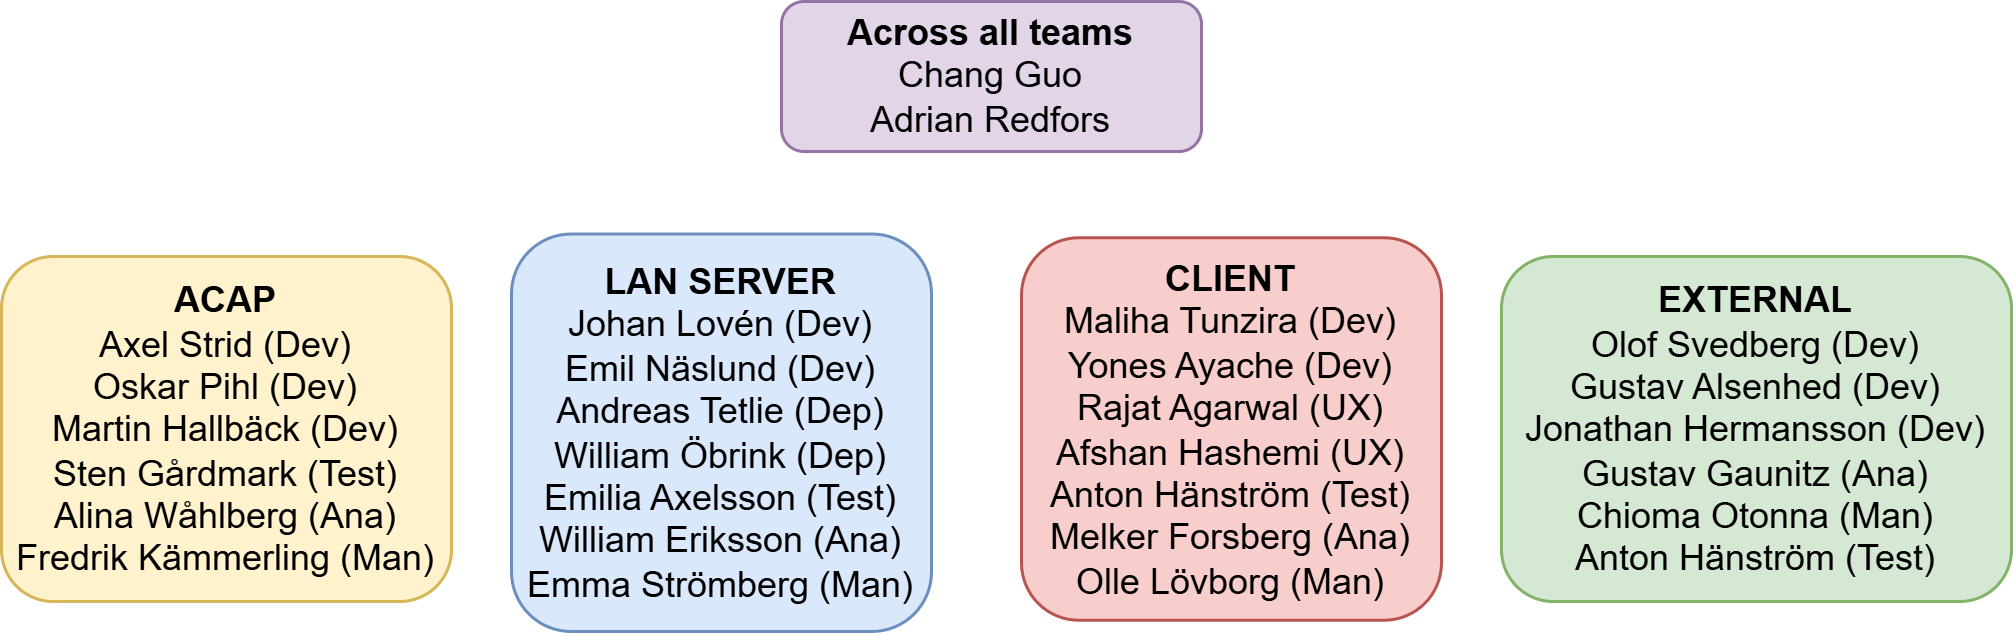
\includegraphics[width=0.5\linewidth]{NewCrossFunctional.drawio.png}
    \caption{Cross-functional teams for Iteration 1 \& 2}
    \label{fig:enter-label}
\end{figure}
    
\subsection{End Users}
The primary end users require efficient alert systems, clear data visualizations, and intuitive controls for managing security incidents. These users of the system will be security professionals, including:
    
\begin{itemize}
    \item Security operators monitoring video feeds and responding to alerts
    \item Security managers overseeing operations and accessing analytical data
    \item System administrators managing access and configurations
\end{itemize}
    

    
\section{Project Constraints}
    
\subsection{Personnel}
The project is constrained by a 160-hour limit per team member. This necessitates careful planning and resource management throughout the project lifecycle. Additionally, team members have other academic commitments inherent to being students, which must be respected and managed alongside project work. This differs from a traditional work environment and requires flexible scheduling and efficient time utilization.
    
\subsection{Timeline}
The timeline of the project requires management of development cycles and regular progress reviews to ensure in-time delivery of project milestones. The project is bound by the following key dates:
    
\begin{tabular}{ll}
    \textbf{Event} & \textbf{Date} \\
    \hline
        Project Start & September 4, 2024 \\
        Tollgate Meeting & September 26, 2024 \\
        Iteration 1 End & October 11, 2024 \\
        Iteration 2 End & November 8, 2024 \\
        Iteration 3 End & November 22, 2024 \\
        Iteration 4 End & December 6, 2024 \\
        VSSE (Final Presentation) & December 12, 2024 \\
\end{tabular}

    
\subsection{Resources}
The project operates without a dedicated budget, which significantly impacts available resources. Key constraints include:
    
\begin{itemize}
    \item Reliance on virtual environments for large-scale testing scenarios
    \item No funds for third-party software licenses, AI models, or cloud computing resources
    \item Time constraints for students in our company
    \item Time limitations for learning new technologies or frameworks
\end{itemize}
    
To address these constraints, the team will focus on open-source tools, efficient resource utilization, and prioritization of core functionalities. Open communication with Axis Communications and the course adminstration will be maintained for any critical support or resources needed for project success.
    
\section{Deliverables}
The project will result in both product and documentation deliverables, each crucial to the success of the security surveillance solution.
    
\subsection{Product Deliverables}
    
The core of our solution will comprise of several connected components:
    
   % @Chioma, please confirm the deliverables from development team
\begin{description}
    \item[Video Analysis Engine:] For processing video feeds and detecting anomalies.
    \item[Alert Management System:] For generating and managing security alerts.
    \item[Operator Interface:] A dashboard for security personnel to monitor and respond to alerts.
    \item[Camera Integration Module:] For integration with Axis camera systems.
    % \item[Data Visualization Tool] Need to confirm if this is a required component
\end{description}
    
    % Additional components may be needed based on specific project requirements - Fredrik Kämmerling?
    
\subsection{Documentation Deliverables}

To support our product and ensure its proper implementation and use, we will produce the following key documents:

\begin{center}
\begin{tabular}{|p{0.3\textwidth}|p{0.6\textwidth}|}
    \hline
    \textbf{Document} & \textbf{Description} \\
    \hline
    Architecture Notebook & Overview of system architecture and design rationale \\
    \hline
    Project Backlog & Listing of functional and non-functional system requirements \\
    \hline
    Test Plan & Outline of testing strategies and procedures \\
    \hline
    Software Quality Assurance Plan & Documentation of quality standards and processes \\
    \hline
    Customer Requirements Specification & Documentation of customer requirements and expectations \\
    \hline
\end{tabular}
\end{center}

\section{Project Schedule}

Our project timeline is structured to ensure steady progress and regular delivery of value. Work is divided into four key iterations.

\subsection{Iteration Plan}
Presented below are the dates and focus areas of each iteration: 
\begin{center}
    \begin{tabular}{|c|l|l|}
        \hline
        \textbf{Iteration} & \textbf{Dates} & \textbf{Focus} \\
        \hline
        0 (Tollgate) & Sept 13 - Sept 26 & Company Overview, Requirements Specification, Architectural Description, Milestone Plan, Acceptance Testing Plan, UX \& Organizational Structure \\
        \hline
        1 & Sept 30 - Oct 11 & System Integration, Database Setup, Initial Client-Facing Website Development, SQA Plan, Test Plan, CI/CD Plan \\
        \hline
        2 & Oct 14 - Nov 8 & Alarm Management, Scheduling System Development, Continued Client-Facing Website Development \\
        \hline
        3 & Nov 11 - Nov 22 & Continued Scheduling System Development, Alarm Confidence Level, Multi-Camera Support \\
        \hline
        4 & NOv 22 - Dec 6 & Data Compliance \& GDPR Management, Scalability Enhancement, Final Presentation Preparation \\
        \hline
    \end{tabular}
    \end{center}


\subsection{Key Milestones}

Our project timeline contains the following key events:

\begin{center}
\begin{tabular}{|l|c|}
    \hline
    \textbf{Milestone} & \textbf{Date} \\
    \hline
    Project Kickoff & September 4, 2024 \\
    Tollgate Meeting & September 26, 2024 \\
    Iteration 1 End & October 11, 2024 \\
    Iteration 2 End & November 8, 2024 \\
    Iteration 3 End & November 22, 2024 \\
    VSSE (Final Presentation) & December 12, 2024 \\
    \hline
\end{tabular}
\end{center}


\begin{figure}[h]
    \centering
    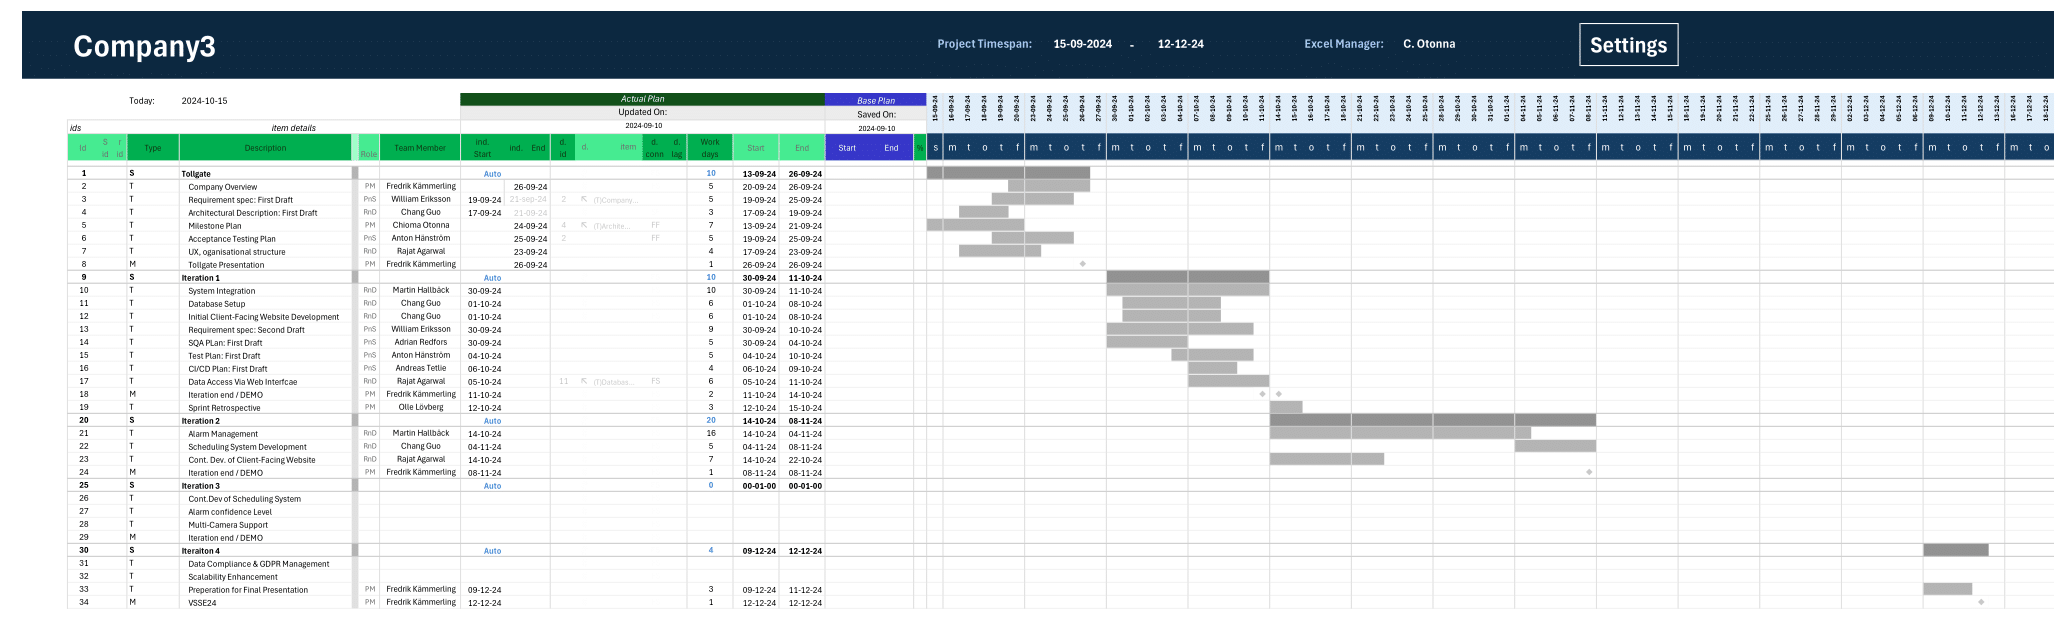
\includegraphics[width=\textwidth]{Milestone Plan-1.png}
    \caption{Project Milestone Plan and Gantt Chart}
    \label{fig:milestone-plan}
\end{figure}

\section{Quality Objectives}

Quality is at the heart of our development process, encompassing both the product we deliver and the methods we employ to create it.

\subsection{Product Quality}

Our security surveillance solution aims to meet the following quality benchmarks:

% Need to confirm specific quality metrics with stakeholders
% @Emma: Please confirm the quality metrics
\begin{itemize}
    \item Achieve high system uptime during operational hours.
    \item Generate alerts within a specified time frame of incident detection.
    \item Maintain a low false positive rate for security alerts.
    \item Design an intuitive interface for efficient user interaction.
    \item Support multiple simultaneous camera feeds.
\end{itemize}


\subsection{Process Quality}

% @Chioma: Please confirm the rnd side of things here 
To ensure an effective development process, we commit to:

Adhering to iterative development methodologies, with regular reviews and retrospectives to continuously improve our processes. Our documentation will be updated at the conclusion of each iteration to reflect the latest project state.

Implementing a comprehensive Quality Assurance plan that is iterative in nature, with a focus on continuous improvement. This plan spans across both the Research and Development (RnD) and Product and Sales (PnS) departments, covering all iterations. Key roles and responsibilities are outlined in Table \ref{tab:qa-responsibilities}.

\begin{table}[h]
\centering
\caption{Quality Assurance Roles and Responsibilities}
\label{tab:qa-responsibilities}
\begin{tabular}{|l|l|}
\hline
\textbf{Role} & \textbf{Responsibility} \\
\hline
Product and Sales Line Manager & Overall QA plan \\
Technical Writer & Document structure and version control \\
Testing Lead & Testing strategy and bug tracking \\
Analysis Lead & Traceability \\
Deployment Lead & Continuous integration and delivery \\
Process Manager & Internal quality practices and change management \\
Architecture & Future development and operations considerations \\
\hline
\end{tabular}
\end{table}

Utilizing a Continuous Integration and Continuous Delivery (CI/CD) pipeline to automate the build, test, and deployment processes. Our CI/CD pipeline, managed through GitLab CI, includes automated testing, Docker image building, and deployment to a Kubernetes cluster hosted in Azure. This approach ensures consistent code quality, frequent integration, and reliable deployments.

Maintaining code quality through review processes before merging major features into our main codebase. We aim for comprehensive automated testing coverage for all new code, ensuring reliability.

Soliciting regular stakeholder feedback, with dedicated sessions throughout the project. This approach ensures that we remain aligned with stakeholder expectations and can adapt to changing requirements or priorities.

Conducting sprint retrospectives after each iteration to evaluate our practices and processes, as outlined in our quality management plan. These retrospectives will cover areas such as document version handling, internal test cases, code refactoring, methods of communication, and the retrospective process itself.

Implementing a feedback loop system where all employees are encouraged to provide continuous feedback and recommendations on quality assurance practices to their Lead, Line Manager, or the Project Manager.

Through these quality objectives and processes, we aim to deliver a security surveillance solution that maintains high standards of quality throughout its development lifecycle.